%% BioMed_Central_Tex_Template_v1.06
%%                                      %
%  bmc_article.tex            ver: 1.06 %
%                                       %

%%IMPORTANT: do not delete the first line of this template
%%It must be present to enable the BMC Submission system to 
%%recognise this template!!

%%%%%%%%%%%%%%%%%%%%%%%%%%%%%%%%%%%%%%%%%
%%                                     %%
%%  LaTeX template for BioMed Central  %%
%%     journal article submissions     %%
%%                                     %%
%%         <14 August 2007>            %%
%%                                     %%
%%                                     %%
%% Uses:                               %%
%% cite.sty, url.sty, bmc_article.cls  %%
%% ifthen.sty. multicol.sty		   %%
%%				      	   %%
%%                                     %%
%%%%%%%%%%%%%%%%%%%%%%%%%%%%%%%%%%%%%%%%%


%%%%%%%%%%%%%%%%%%%%%%%%%%%%%%%%%%%%%%%%%%%%%%%%%%%%%%%%%%%%%%%%%%%%%
%%                                                                 %%	
%% For instructions on how to fill out this Tex template           %%
%% document please refer to Readme.pdf and the instructions for    %%
%% authors page on the biomed central website                      %%
%% http://www.biomedcentral.com/info/authors/                      %%
%%                                                                 %%
%% Please do not use \input{...} to include other tex files.       %%
%% Submit your LaTeX manuscript as one .tex document.              %%
%%                                                                 %%
%% All additional figures and files should be attached             %%
%% separately and not embedded in the \TeX\ document itself.       %%
%%                                                                 %%
%% BioMed Central currently use the MikTex distribution of         %%
%% TeX for Windows) of TeX and LaTeX.  This is available from      %%
%% http://www.miktex.org                                           %%
%%                                                                 %%
%%%%%%%%%%%%%%%%%%%%%%%%%%%%%%%%%%%%%%%%%%%%%%%%%%%%%%%%%%%%%%%%%%%%%


\documentclass[10pt]{article}    



% Load packages
\usepackage{cite} % Make references as [1-4], not [1,2,3,4]
\usepackage{url}  % Formatting web addresses  
\usepackage{ifthen}  % Conditional 
\usepackage{multicol}   %Columns
\usepackage{hhline}
\usepackage[utf8]{inputenc} %unicode support
\usepackage{graphicx}
\usepackage{verbatim}
\usepackage{amsmath}
%\usepackage[applemac]{inputenc} %applemac support if unicode package fails
%\usepackage[latin1]{inputenc} %UNIX support if unicode package fails
\urlstyle{rm}
 
 
%%%%%%%%%%%%%%%%%%%%%%%%%%%%%%%%%%%%%%%%%%%%%%%%%	
%%                                             %%
%%  If you wish to display your graphics for   %%
%%  your own use using includegraphic or       %%
%%  includegraphics, then comment out the      %%
%%  following two lines of code.               %%   
%%  NB: These line *must* be included when     %%
%%  submitting to BMC.                         %% 
%%  All figure files must be submitted as      %%
%%  separate graphics through the BMC          %%
%%  submission process, not included in the    %% 
%%  submitted article.                         %% 
%%                                             %%
%%%%%%%%%%%%%%%%%%%%%%%%%%%%%%%%%%%%%%%%%%%%%%%%%                     


%\def\includegraphic{}
%\def\includegraphics{}



\setlength{\topmargin}{0.0cm}
\setlength{\textheight}{21.5cm}
\setlength{\oddsidemargin}{0cm} 
\setlength{\textwidth}{16.5cm}
\setlength{\columnsep}{0.6cm}


%%%%%%%%%%%%%%%%%%%%%%%%%%%%%%%%%%%%%%%%%%%%%%%%%%
%%                                              %%
%% You may change the following style settings  %%
%% Should you wish to format your article       %%
%% in a publication style for printing out and  %%
%% sharing with colleagues, but ensure that     %%
%% before submitting to BMC that the style is   %%
%% returned to the Review style setting.        %%
%%                                              %%
%%%%%%%%%%%%%%%%%%%%%%%%%%%%%%%%%%%%%%%%%%%%%%%%%%
 

%Review style settings
%\newenvironment{bmcformat}{\begin{raggedright}\baselineskip20pt\sloppy\setboolean{publ}{false}}{\end{raggedright}\baselineskip20pt\sloppy}

%Publication style settings
%\newenvironment{bmcformat}{\fussy\setboolean{publ}{true}}{\fussy}

%New style setting

% Begin ...
\begin{document}


%%%%%%%%%%%%%%%%%%%%%%%%%%%%%%%%%%%%%%%%%%%%%%
%%                                          %%
%% Enter the title of your article here     %%
%%                                          %%
%%%%%%%%%%%%%%%%%%%%%%%%%%%%%%%%%%%%%%%%%%%%%%

%\title{A Probablistic Space-efficient Method of Obtaining Solid Kmers with An Appliction of Error Correction}
\title{Lighter: fast and memory-efficient error correction without counting}

%%%%%%%%%%%%%%%%%%%%%%%%%%%%%%%%%%%%%%%%%%%%%%
%%                                          %%
%% Enter the authors here                   %%
%%                                          %%
%% Ensure \and is entered between all but   %%
%% the last two authors. This will be       %%
%% replaced by a comma in the final article %%
%%                                          %%
%% Ensure there are no trailing spaces at   %% 
%% the ends of the lines                    %%     	
%%                                          %%
%%%%%%%%%%%%%%%%%%%%%%%%%%%%%%%%%%%%%%%%%%%%%%


\author{Li Song$^1$
  Liliana Florea$^2$
  Ben Langmead$^{*3}$
}

%%%%%%%%%%%%%%%%%%%%%%%%%%%%%%%%%%%%%%%%%%%%%%
%%                                          %%
%% Enter the authors' addresses here        %%
%%                                          %%
%%%%%%%%%%%%%%%%%%%%%%%%%%%%%%%%%%%%%%%%%%%%%%

\maketitle

%%%%%%%%%%%%%%%%%%%%%%%%%%%%%%%%%%%%%%%%%%%%%%
%%                                          %%
%% The Abstract begins here                 %%
%%                                          %%  
%% Please refer to the Instructions for     %%
%% authors on http://www.biomedcentral.com  %%
%% and include the section headings         %%
%% accordingly for your article type.       %%   
%%                                          %%
%%%%%%%%%%%%%%%%%%%%%%%%%%%%%%%%%%%%%%%%%%%%%%


\begin{abstract}
        % Do not use inserted blank lines (ie \\) until main body of text.
\emph{Lighter} is a fast and memory-efficient tool for correcting sequencing errors in high-throughput sequencing datasets.
\emph{Lighter} avoids counting $k$-mers in the sequencing reads.
Instead, it uses a pair of Bloom filters, one populated with a sample of the input $k$-mers and the other populated with $k$-mers likely to be correct based on a statistical test.
As long as the sampling fraction is adjusted in inverse proportion to the dataset's average coverage, the Bloom filter size can be held constant while maintaining near-constant accuracy.
\emph{Lighter} is easily applied to very large sequencing datasets.  It uses no secondary storage, and is both faster and more memory-efficient than competing approaches while achieving comparable accuracy.
\emph{Lighter} is free open source software available from \url{https://github.com/mourisl/Lighter/}.
\end{abstract}


%%%%%%%%%%%%%%%%%%%%%%%%%%%%%%%%%%%%%%%%%%%%%%
%%                                          %%
%% The Main Body begins here                %%
%%                                          %%
%% Please refer to the instructions for     %%
%% authors on:                              %%
%% http://www.biomedcentral.com/info/authors%%
%% and include the section headings         %%
%% accordingly for your article type.       %% 
%%                                          %%
%% See the Results and Discussion section   %%
%% for details on how to create sub-sections%%
%%                                          %%
%% use \cite{...} to cite references        %%
%%  \cite{koon} and                         %%
%%  \cite{oreg,khar,zvai,xjon,schn,pond}    %%
%%  \nocite{smith,marg,hunn,advi,koha,mouse}%%
%%                                          %%
%%%%%%%%%%%%%%%%%%%%%%%%%%%%%%%%%%%%%%%%%%%%%%

% The idea of using a Bloom filter to store the solid k-mers is not new; CUDA-EC does this
% What's our story w/r/t choosing k-mer length?

\section*{Introduction}
The cost and throughput of DNA sequencing have improved rapidly in the past several years \cite{glenn2011field}, with recent advances reducing the cost of sequencing a single human genome at 30-fold coverage to around \$1,000 \cite{1kgenomeforreal}.
With these advances has come an explosion of new software for analyzing large sequencing datasets.
Sequencing error correction is a basic need for many of these tools.
Removing errors at the outset of an analysis can improve accuracy of downstream tools such as variant callers \cite{kelley2010quake}.
Removing errors can also improve the speed and memory-efficiency of downstream tools, particularly for analyses involving de novo assembly with De Bruijn graphs since the graph's size increases with the number of distinct $k$-mers in the dataset \cite{pevzner2001eulerian, chaisson2004fragment}.

To be useful in practice, error correction software must make economical use of time and memory even when input datasets are extremely large (billions of reads) and when the genome under study is also large (billions of nucleotides).
Several methods have been proposed, covering a wide tradeoff space between accuracy, speed and memory- and storage-efficiency.
SHREC \cite{schroder2009shrec} and HiTEC \cite{ilie2011hitec} build a suffix index of the input reads and locate errors by finding instances where a substring is followed by a character less often than expected.
Coral \cite{salmela2011correcting} and ECHO \cite{kao2011echo} find overlaps among reads and use the resulting multiple alignments to detect and correct errors.
Reptile \cite{yang2010reptile} and Hammer \cite{medvedev2011error} detect and correct errors by examining each $k$-mer's neighborhood in the dataset's $k$-mer Hamming graph.

% Citations
% Quake: 149, used in GAGE, assemblathon, 
% SHREC: 68, none seem to be users
% Reptile: 52, no obvious users
% HiTEC: 46, none seem to be users
% ECHO: 37, a handful seem to be users
% Hammer: 35, 
% Coral: 34, no obvious users
% CUDA-EC: 33, no obvious users
% DecGPU: 15
% Musket: 8
% BLESS: 0
% Turtle: 1

The most practical and widely used error correction methods descend from the spectral alignment approach introduced in the earliest De Bruijn graph based assemblers \cite{pevzner2001eulerian, chaisson2004fragment}.
These methods count the number of times each $k$-mer occurs (its \emph{multiplicity}) in the input reads, then apply a threshold such that reads with multiplicity exceeding the threshold are considered \emph{solid}.
Solid $k$-mers are unlikely to have been altered by sequencing errors.
$k$-mers with low multiplicity (\emph{weak} $k$-mers) are systematically edited into solid $k$-mers using a dynamic-programming solution to the spectral alignment problem \cite{pevzner2001eulerian, chaisson2004fragment} or, more often, a fast heuristic approximation.
Quake \cite{kelley2010quake}, the most widely used error correction tool, uses a hash-based $k$-mer counter called Jellyfish \cite{marccais2011fast} to determine which $k$-mers are solid.
CUDA-EC \cite{shi2010parallel} was the first to use a Bloom filter as a space-efficient alternative to hash tables for counting $k$-mers and for representing the set of solid $k$-mers.
More recent tools such as Musket \cite{liu2013musket} and BLESS \cite{heo2014bless} use a combination of Bloom filters and hash tables to count $k$-mers or to represent the set of solid $k$-mers.

\emph{Lighter} (LIGHTweight ERror corrector) is also in the family of spectral alignment methods, but differs from previous approaches in that it avoids counting $k$-mers.
Rather than count $k$-mers, \emph{Lighter} samples $k$-mers randomly, storing the sample in a Bloom filter.
\emph{Lighter} then uses a statistical test applied to each position of each read to compile a set of solid $k$-mers, stored in a second Bloom filter.
These two Bloom filters are the only sizable data structures used by \emph{Lighter}.

\emph{Lighter}'s crucial advantage is that its parameters can be set such that the memory footprint and the accuracy of the approach are near-constant with respect to coverage.
That is, no matter how deep the coverage, \emph{Lighter} can allocate the same sized Bloom filters and achieve nearly the same (a) Bloom filter occupancy, (b) Bloom filter false positive rate, and (c) error correction accuracy.
\emph{Lighter} does this without using any disk space or other secondary memory.
This is in contrast to BLESS and Quake/Jellyfish, which use secondary memory to store some or all of the $k$-mer counts.
\emph{Lighter}'s accuracy is comparable to competing tools, as we show both in simulation experiments where false positives and false negatives can be measured, and in real-world experiments where read alignment scores and assembly statistics can be measured.  
\emph{Lighter} is also very simple and fast, faster than all other tools tried in our experiments.
These advantages make \emph{Lighter} quite practical compared to previous counting-based approaches, all of which require an amount of memory or secondary storage that increases with depth of coverage.



%\emph{Lighter} makes a series of three passes over the input reads.  The first pass obtains a sample of the k-mers present in the input reads, storing the sample in a Bloom filter A.  The second pass uses Bloom filter A to identify ``solid'' k-mers and stores these in Bloom filter B.  The third pass uses Bloom filter B to detect and correct errors in the input reads.

%One important way to study a species is to sequence its genome and analyze its DNA. The need to understand the genome stimulates the rapid development of DNA sequencing technologies. The output of the DNA sequencing is usually an enormous volume of short fragments from the genome. With these small fragments, computational biologists are able to design complicated methods to reconstruct the original genome by assembling or to detect the mutations from the known reference genome by aligning.

%The volume of the data is so huge that if we align them to the genome, each position is covered by a bunch of reads which is called the coverage. However, the short fragments are not perfect and usually contain a small number of sequecing errors. This affects one of the most important preprocessing stages for the data --- kmer counting, where a kmer is a nucleutide sequence of size k. If there is no sequencing error, all the kmers are from the genome, which are called solid kmers, and its quantity are bounded by the genome size instead of the coverage. This is not true in practice due to the sequecing errors and if the coverage is high enough, like what the sequecing technology gives us nowadays, the kmers containing sequencing errors will dominate the space consumption. To alleviate the impact from those non-solid kmers, various methods have been proposed, like BFcounter[cite]. These methods still suffer from the problem that the space consumption scales up with the coverage. In this paper, we propose a probablitic methods of obtaining solid kmers whose space complexity does not depend on the coverage.

%One immediate applicaiton using the information of solid kmers is error correction. Error correction is very important for the De Brujin graph based genome assemblers to save the memory usage. There are mainly three categories methods for error correction[cite], and converting all the kmers to solid kmers is one of them and is particularly successful for Illumina reads where the read errors are mainly substitutions. There are currently many programs for error corrections, and some of them are highlighted for their low memory usage, like Musket[cite] and Bless[cite]. With the help of our method of obtainig solid kmers and the bloom filters which is a compact probabilitc data structure, we also propose the program Lighter(LIGHT-weight ERror correction) that can do error correction with very small memory footprint and no extra disk consumption.

\section*{Method}
Lighter's workflow is illustrated in Figure \ref{fig:lighter_framework}. Lighter makes three passes over the input reads.  The first pass obtains a sample of the k-mers present in the input reads, storing the sample in Bloom filter A.  The second pass uses Bloom filter A and a hypothesis test to identify solid k-mers, which it stores in Bloom filter B.  The third pass uses Bloom filter B and a greedy procedure to correct errors in the input reads.

\begin{figure}[h!]
\begin{center}
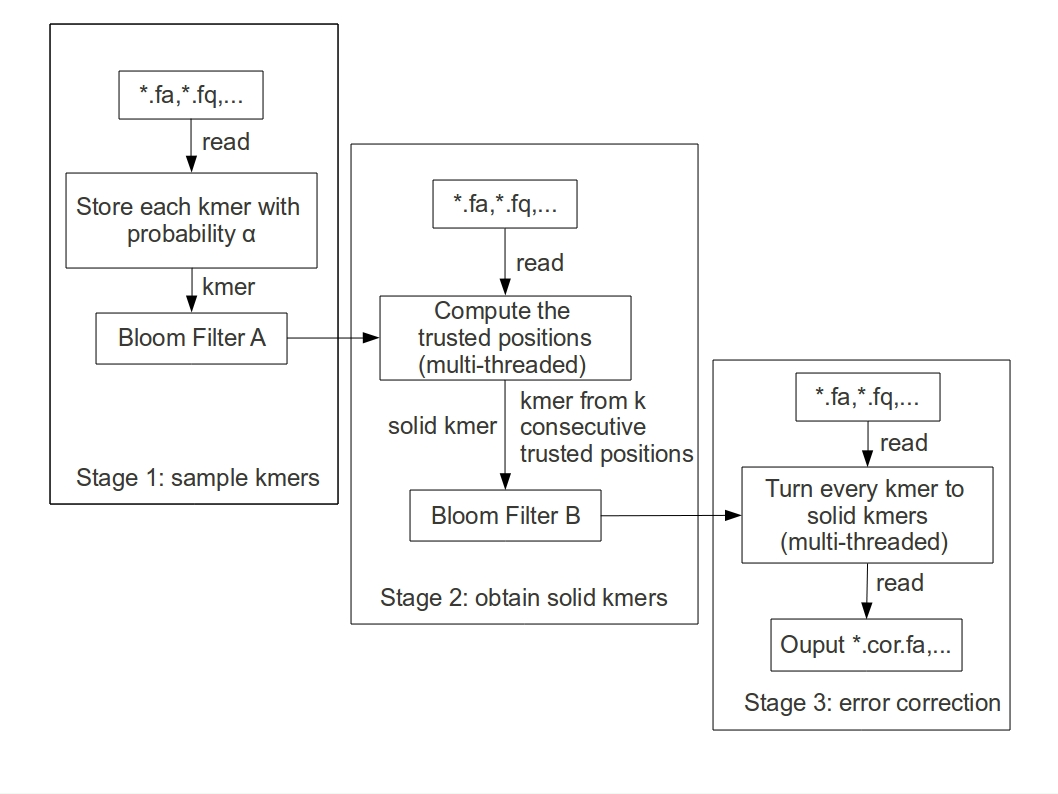
\includegraphics[width=0.75\textwidth]{lighter_framework.jpg}
\caption{The framework of Lighter\label{fig:lighter_framework}}
\end{center}
\end{figure}

\subsection*{Bloom filter}
A Bloom filter \cite{bloom1970space} is a compact probabilistic data structure representing a set.  It consists of an array of $m$ bits, initialized to 0.  To add an object $o$, $h$ independent hash functions $H_0(o), H_1(o),...,H_{h-1}(o)$ are applied.  Each maps $o$ to an integer in $[0, m)$ and the corresponding $h$ array bits are set to 1. To test if object $q$ is a member, the same hash functions are applied to $q$.  $q$ is a member if all corresponding bits are set to 1.  A false positive occurs when the corresponding bits are set to 1 ``by coincidence,'' that is, because of objects besides $q$ that were added previously.  Assuming the hash functions map objects to bit array elements with equal probability, the Bloom filter's false positive rate is approximately $(1-e^{-h\frac{n}{m}})^h$, where $n$ is the number of distinct objects added, which we call the \emph{cardinality}.  Given $n$, which is usually determined by the dataset, $m$ and $h$ can be adjusted to achieve a desired false positive rate.  Lower false positive rates can come at a cost, since greater values of $m$ require more memory and greater values of $k$ require more hash function calculations.  Many variations on Bloom filters have been proposed that additionally permit compression of the filter, storage of count data, representation of maps in addition to sets, etc \cite{tarkoma2012theory}.  Bloom filters and variants thereon have been applied in various bioinformatics settings, including assembly \cite{pell2012scaling}, compression \cite{jones2012compression}, k-mer counting \cite{melsted2011efficient}, and error correction \cite{shi2010parallel}.

By way of contrast, another way to represent a set is with a hash table.  Hash tables do not yield false positives, but Bloom filters are far smaller.  Whereas a Bloom filter is an array of bits, a hash table is an array of buckets, each large enough to store a pointer, key, or both.  If chaining is used, lists associated with buckets incur additional overhead.  While the Bloom filter's small size comes at the expense of false positives, these can be tolerated in many settings including in error correction.

As Figure \ref{fig:lighter_framework} shows, the efficiency of bloom filter affects the running time of Lighter a lot. For a standard Bloom filter, the $h$ hash functions may map $o$ to any places in the bit array. The bit array is usually very large, so all the $h$ accesses will likely to cause cache miss. In [cite], the authors proposed blocked Bloom filter which can decrease the number of cache misses. Given a block size $b$, it will use $H_0(o)$ to decide the start position on the bit array, and then map $H_0(o), H_1(o),...,H_{h-1}(o)$ onto the block starting from that position. It choose $b$ about the size of a cache line, then the $h$ accesses will not cause $h$ cache misses. The drawback of using blocked Bloom filter is that we have to use a bit larger $h$ and $m$ to have the same FPR when using the standard bloom filter. To estimate the FPR of blocked Bloom filter, we can consider each of the possible $m-b+1$ blocks. for the $i$-th block, the FPR within this block is $(b'_i/b)^h$, where $b'_i$ is the number of bits set to 1 in block $i$. So the overall FPR is $\displaystyle\frac{\sum_i (b'_i/b)^h}{m-b+1}$.

In our method, the objects to be stored in the Bloom filters are k-mers.  Because we would like to treat genome strands equivalently for counting purposes, we will always \emph{canonicalize} a k-mer before adding it to, or using it to query a Bloom filter.  A canonicalized k-mer is either the k-mer itself or its reverse complement, whichever is less than or equal to the other.

% What do we do with k-mers with ambiguous nucleotides?

\subsection*{First pass}

\paragraph{Sampling.}  Consider a k-mer drawn from a read.  We say the k-mer is \emph{incorrect} if its sequence has been altered by one or more sequencing errors.  Otherwise it is \emph{correct}.  Others have noted that, given a dataset with deep and uniform coverage, incorrect k-mers occur rarely while correct k-mers occur many times, proportionally to coverage \cite{pevzner2001eulerian, chaisson2004fragment}.

In the first pass over the input reads, Lighter examines each k-mer of each read, canonicalizing and storing it in Bloom filter $A$ with probability $\alpha$, where $\alpha$ is an adjustable parameter.  Say a particular k-mer sequence occurs a total of $N_k$ times in the dataset.  If the $\alpha$ filter discards all $N_k$ occurrences, the k-mer is never added to $A$ and $A$'s cardinality is reduced by one.  Thus, reducing $\alpha$ in turn reduces $A$'s cardinality.  Because correct k-mers are more numerous, incorrect k-mers tend to be discarded from $A$ before correct k-mers as $\alpha$ decreases.

%In the rest of the method, it is beneficial for $A$ to include as many correct and as few incorrect k-mers as possible, though the method is still robust when $A$ contains some incorrect and lacks some correct k-mers.

%Assume that, regardless of average coverage, there is always a value of $\alpha$ for which $n \approx G$, where $G$ is the length of the sequenced genome, and the k-mers stored in $A$ are almost all correct.  If this is the case, we can fix $m$ and $h$ and adjust $\alpha$ to achieve a desired false positive rate.  This is in contrast to fixing $n$ and adjusting $m$ and $h$.  We do not argue here that the assumption is true, but we do show later that in practice $\alpha$ can be set to achieve desirable $m$, $k$ and false positive rate for a range of coverage levels.

%In other words, the size of $A$ depends almost only on the genome size. For $75\times$ coverage sequence data, we can let $\alpha$ be $0.05$.

\subsection*{Second pass}

\paragraph{Finding trusted read positions.} 
A read position overlaps up to $x$ $k$-mers where $1\le x\le k$. If the position was altered by a sequencing error, the overlapping $k$-mers are incorrect and likely weak. These weak $k$-mers are not likely to be sampled by Lighter in the first pass, so we can set a threshold and for this position if the number of $k$-mers that are stored in Bloom filter $A$ is less than this threshold we say this position is untrusted, otherwise we say it is trusted. We call the comparison against the threshold as a test case. For two test cases, if their $x$ $k$-mers are the same, their test results are the same and we should say they are the same the test case. 

In Lighter, we set the threshold according to the binomial distribution $b_0\sim Binom(P^*(\alpha), x)$, where $P^*(\alpha)$ is some probability depending on the value of $\alpha$ and will be defined later. If $y$ is the minimum integer that $p(b_0>=y)<0.05$, then we set the threshold $y'=y+1$. To define $P^*(\alpha)$, firstly we define $P(\alpha)=1-(1-\alpha)^{f(\alpha)}$, where $f(\alpha)=max\{2,0.1/\alpha\}$. So 
$$P^*(\alpha)=P(\alpha)+\beta-\beta P(\alpha)$$
where $\beta$ is the false positive rate of Bloom filter $A$.

The intuition behind this threshold is that we assume the multiplicity of a weak kmer is at most $f(\alpha)$. If a position is wrong, the $x$ $k$-mers' multiplicity is likely to be no more than $f(\alpha)$, and the number of them showing up in Bloom filter $A$ is bounded by $b0$. We do not want such position be regarded as trusted, so we set a high-enough threshold so we can say this position is untrusted.

One property of this threshold is that when $\alpha$ is small, $P(\alpha/z)=1-(1-\alpha/z)^{0.1z/\alpha}\approx 1-(1-\alpha)^{0.1/\alpha}=P(\alpha)$, where $z$ is some constant larger than 1 and we applied the approximation that $(1-\alpha/z)^z\approx 1-\alpha$.

%Let $m(r)$ denote $k$-mer $r$'s multiplicity.  Let $P(\alpha, m(r))$ be the probability that $r$ is added to Bloom filter A given sampling rate $\alpha$:
%$$P(\alpha, m(r)) = 1-(1-\alpha)^{m(r)}$$

%When we query Bloom filter $A$, whether we get a positive response depends both on $P(\alpha, m(r))$ and on the filter's false positive rate, which we call $\beta$.  The probability $P^*(\alpha, m(r))$ of getting a positive response when querying for $r$ in $A$ is:

%$$P^*(\alpha, m(r))=P(\alpha, m(r))+\beta-P(\alpha, m(r))\beta$$

%Say $\gamma$ is the expected multiplicity of a correct $k$-mer.  We call a $k$-mer $r$ weak if $m(r)$ is much less than $\gamma$. Specifically, we say $r$ is weak if $m(r) \leq \gamma'$, where $\gamma'=\gamma/c$ and $c$ is a constant we must choose. We can bound the probability that a weak $k$-mer is added to Bloom filter A given sampling rate $\alpha$:

%$$P(\alpha, 1) \leq P_{weak}(\alpha) \leq P(\alpha, \gamma')$$

%The lower bound corresponds to the case where all weak $k$-mers have multiplicity 1 and the upper bound corresponds to the case where all weak $k$-mers have multiplicity $\gamma'$.  Additionally taking false positive rate into account, we can bound the probability $P^*_{weak}(\alpha)$ that the Bloom filter gives a positive response when queried with a weak $k$-mer:

%$$P^*(\alpha, 1) \leq P^*_{weak}(\alpha) \leq P^*(\alpha, \gamma')$$

%In the following we conservatively assume $P_{weak}(\alpha) = P(\alpha, \gamma')$ and $P^*_{weak}(\alpha) = P^*(\alpha, \gamma')$.


%:  above by $P(\alpha, \gamma')$ and below by .

%For the $k$-mers containing sequencing errors, we will call it true weak kmers. In practice, the multiplicity of most true weak $k$-mers grows much slower when we increase $\gamma$ namely increasing the coverage. So $\gamma'$ will overestimate the mulitplicity of true weak $k$-mers a lot. 

 %To determine whether a position is incorrect, we perform a one-tailed hypothesis test where the null hypothesis is that all overlapping $k$-mers are weak.  For a weak $k$-mer, a positive response from Bloom filter A happens with probability $P^*(\alpha, \gamma')$ (conservatively), and the number of overlapping $k$-mers yielding a positive response follows a binomial distribution with success probability $P^*(\alpha, \gamma')$ and number of trials $x$.  Let $y \leq x$ be the actual number of $k$-mers overlapping the read position that appear in A and let $y'$ be the minimum integer value for $y$ such that the hypothesis test P value is less than 0.005.  If $y \geq y'$, we reject the null hypothesis and the read position is called \emph{trusted}, otherwise it is called \emph{untrusted}. 

%Framing the problem as a hypothesis test is convenient since it naturally handles the case where $x<k$.  $y'$ thresholds can be pre-calculated for efficiency.

%A one-tail hypothesis testing. The null hypothesis is that this position is wrong and the p-value can be get from test again $(x,P^*(\alpha, \gamma'))$ using the actual number of kmers in $A$ containing that position. We use $y$ to denote this actual number of kmers. In our method, suppose $y'$ is the first number whose p-value is smaller than 0.005, if $y>y'$, we reject the null hypothes and the position is trusted. The benefit of using hypothesis testing instead of using a fixed threshold is that we can handle the case where $x<k$ in a consistent way and it can tolerate the ill-chosen $\alpha$. Notice that, the position near the left and right boundary or near an error may never be trusted.

\paragraph{Finding solid $k$-mers.}  Once all positions in a read have been marked \emph{trusted} or \emph{untrusted}, we scan the read and find all places where $k$ trusted positions are in a row.  The $k$-mer made up by those positions is likely solid, and so we add it to Bloom filter B.  

%After marking each positions, if there are consecutive k trusted positions, we store the corresponding kmer, which is likely a solid $k$-mer, in another bloom filter $B$. Because these kmers are likely from the real genome, the size of $B$ also only depends on the genome size. 

\paragraph{Scaling with coverage.}  We now show that we can keep the space consumption almost constant by adjust $\alpha$ according to the coverage. If the coverage increases by factor z, we can set $\alpha_2=\alpha_1/z$, and we will show that it almost keeps the performance of the hypothesis testing in the next.

We use a simple model of the sequencing process, including errors.  Let $K$ be the total number of $k$-mers obtained by the sequencer.  Let $\epsilon$ be the fraction that are incorrect, i.e. altered by at least one sequencing error.  We assume the sequencer obtains correct $k$-mers by sampling independently and uniformly from $k$-mers in the genome.  We also assume the number of $k$-mers in the genome is $G$, and that all genomic $k$-mers are distinct.  If $\kappa_c$ is a random variable representing the multiplicity of a correct $k$-mer in the input, $\kappa_c$ has a binomial distribution with success probability $1/G$ and number of trials $(1-\epsilon)K$: $\kappa_c \sim Binom(1/G, (1-\epsilon)K)$. In Lighter, after the sequencer obtained this kmer, it has to be sampled again by the probability of $\alpha$. Let $\kappa'_c$ denotes the randome variable representing the number of times that a correct $k$-mer get sampled by both sequencer and Lighter, so $\kappa'_c \sim Binom(\alpha/G, (1-\epsilon)K)$. This binomial distribution can also be approximated by a Poisson distribution, thus $\kappa'_c \sim Pois(\alpha(1-\epsilon)K/G)$. Simiarly, $\kappa_c\sim Pois((1-\epsilon)K)$.

Similarly, we assume that the sequencer obtains incorrect $k$-mers by sampling independently and uniformly from $k$-mers that are ``close to'' a $k$-mer in the genome.  For example, we might define these to be the set of all $k$-mers with low Hamming distance from some genomic $k$-mer.  If $\kappa_e$ is a random variable representing the multiplicity of an incorrect $k$-mer, $\kappa_e$ has a binomial distribution with success probability $1/H$ for some $H$, and number of trials $\epsilon K$: $\kappa_e \sim Binom(1/H, \epsilon K)$.  It's reasonable to assume $H$ is much larger $G$, but we need not specify $H$ precisely for our analysis. We use $\kappa'_e$ to represent the number of times that an incorrect $k$-mer get sampled by both sequencer and Lighter, and by the same argument $\kappa'_e \sim Pois(\alpha\epsilon K / H)$ and $\kappa_e \sim Pois(\epsilon K / H)$.

Finally, we assume $\epsilon$ does not vary with the depth of sequencing. 

We can show that false positive of Bloom filter $A$ stays almost constant. Suppose we have two scenarios, in scenario I, the sequencer outputs $K_1$ $k$-mers and in scenario II, the sequencer outputs $zK_1$ $k$-mers. If we set $\alpha$ to be $\alpha_1$ in scenario I, then $\alpha_2=\alpha_1/z$ in scenario II. As a result, the distribution of $\kappa'_c$ and $\kappa'_e$ do not change in scenario II and are $Pois(\alpha_1(1-\epsilon)K_1)$ and $Pois(\alpha_1\epsilon K_1 / H)$ repsectively. The number of correct $k$-mer get stored in Bloom filter $A$ is $Gp(\kappa'_c\ge 1)$ and the number of incorrector $k$-mer stored in Bloom filter $A$ is $Hp(\kappa'_e\ge 1)$. These two numbers are the same in scenarios I and II, thus the occupancy rate and the false positive rate of Bloom filter $A$ stays almost the same.

Secondly, we can show that if a position and its nearby positions are error-free then its probability of setting as trusted does not change. We already showed that when $\alpha$ is small, $P(\alpha_1)\approx P(\alpha_2)$ and the FPR of Bloom filter $A$ is almost the same, hence $P^*(\alpha_1)\approx P^*(\alpha_2)$. So the threshold $y'$ differentiating whether a position is trusted or not is constant when changing the coverage. Let $p_1=\frac{p(\kappa'_c\ge 1)}{p(\kappa_c\ge 1)}$ be the probability of a correct kmer get sampled by both sequencer and Lighter conditioned on it is sampled by the sequencer. The number of $k$-mers covering this position in Bloom filter $A$ follows a binomial distribution $B_1\sim Binom(p_1+\beta-\beta p_1, x)$. In general, $p_1=\frac{1-e^{-\alpha(1-\epsilon) K/G}}{1-e^{-(1-\epsilon) K/G}}\approx 1-e^{-\alpha(1-\epsilon)K/G}$, which is because $(1-\epsilon)K/G$ is a large number and $e^{-(1-\epsilon)K/G}$ is close to 0. As a result, $p_1$ does not change in scenario I and II and is about $1-e^{-\alpha_1(1-\epsilon)K_1/G}$. So the binomial distribution $B_1$ does not change. Moreover, the number of different test cases does not change and the overall positions that get classified as trusted is almost the same when changing the coverage.
 
Thirdly, we show that the number of positions that contain error and are falsely set as trusted position does not cause trouble. For simplicity, we ignore $\beta$, the affect of the false responses from the Bloom filter $A$, for now. Let $p_2=\frac{p(\kappa'_e\ge 1)}{p(\kappa_e\ge 1)}$. And the number of sampled $k$-mers covering this position is roughly a binomial distribution $B_2\sim Binom(p_2, x)$. In general, $p_2=\frac{1-e^{-\alpha\epsilon K/H}}{1-e^{-\epsilon K/H}}$. Since $\epsilon K/H$ is very close to 0, $e^{-\epsilon K/H}\approx 1-\epsilon K/H$. So $p_2\approx \frac{\alpha \epsilon K/H}{\epsilon K/H}=\alpha$. In sceanrio I, $p_2=\alpha_1$; and in scenario II, $p_2=\alpha_1/z$. Since $y'\ge 1$, the upper bound of the probability that we say this position is trusted is $p(B_2\ge 1)=1-(1-p_2)^x\approx xp_2\approx x\alpha$. And $p(B_2\ge 1)$ is decreased by factor $z$ when we increase the coverage. As a result, $p(B_2\ge y')$ should decrease by factor not slower than $z$. In other words, the probability of falsely trusting a position is decreased by factor $z$. After increaing the coverage, we introduce new sequence errors and the total number of different test cases will roughly increase by factor $z$. Therefore, the number of false trusting will stay the same. Another perspective to get is conclusion is that because the total number of weak kmers get stored in Bloom filter $A$ is constant and the number of different test cases increase, for each test case the number of $k$-mers we retrieved from Bloom filter $A$ will decrease. When $\alpha$ gets too small, $\beta$ may dominant the probability. However, in that case, the probability of $B_2\ge y'$ is extremely small, so it does not cause trouble at that time. 

Therefore, the number of $k$-mers coming from the consecutive trusted positions does not increase which means there is no need to increase the size of Bloom filter $B$ when increasing coverage. Also, the analysis showed that the ability of capturing solid kmers remains almost the same when we change $\alpha$ linearly. 

In both table $A$ and $B$, we only store the cannonical form of a kmer, that is the kmer itself or its reverse complement depending on who has smaller lexicographical order. 

In Lighter, user need to specify the value of $\alpha$. A rule of thumb for choosing $\alpha$ is by applying the nearly linear relationship between $1/\alpha$ and the coverage, and in this paper we choose $\alpha=0.05$ when the coverage is $70\times$. So given the coverage $C$, we can set $\alpha$ to $0.05\frac{70}{C}$. 

\subsection*{Third pass: error correction}
To show that our method of getting and storing solid kmers is reliable, we designed an error correction method just using the kmers stored in bloom filter $B$.

The correction is done read by read. For a read of length $|r|$, we have $|r|-k+1$ kmers and $k_i$ denote the kmer starts at position $i$ where $1\le i\le|r|-k+1$. We start the correction by finding a longest consecutive kmers that are stored in $B$, and then do the correction by scanning towards left and right. Since the correction towards left and right are symmetric, we only demonstrate the correction for the right-hand scanning. Ideally, when we move from the solid kmers towards right, the first time we see an weak kmer, say $k_i$, there must be an error at position $i+k-1$. There are three candidates or four(if the position is N) to replace this position. For each candidate, we see how many consecutive kmers is solid starting from $k_i$ with this new character. We choose the candidate creating most solid kmers. Then we resume scanning towards right starting from the next unstored kmer. If none of the candidate makes $k_i$ solid or more than one candidate create most solid kmers, we say position $i+k-1$ is ambiguous and stop there. If $i+k-1$ is far from the end of the read, we do the error correction on the substring from $i+k-1$ to the end of a read.

The scheme of this greedy error correction method is shown in Figure \ref{fig:error_correction}, where we choose found the error because there is no kmer CCGATTC. We choose A to replace C since it gives us most consecutive solid kmers up to the end of the read.

\begin{figure}[h!]
\begin{center}
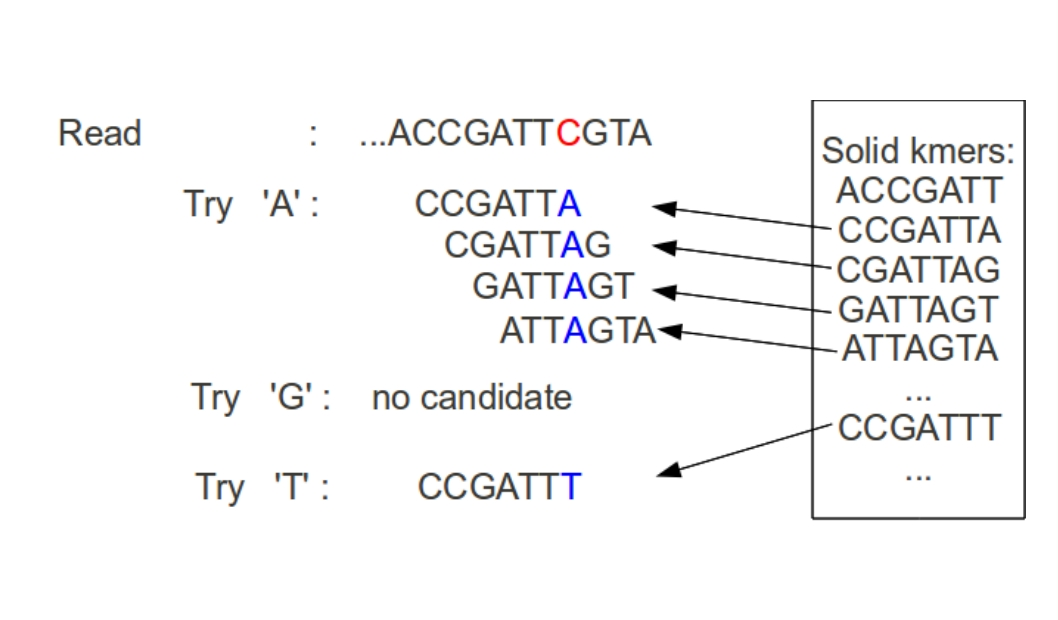
\includegraphics[width=0.75\textwidth]{ErrorCorrection.jpg}
\caption{The framework of Lighter\label{fig:error_correction}}
\end{center}
\end{figure}

\subsection*{Parallization}
As shown in Figure \ref{fig:lighter_framework}, Lighter works in three stages: sampling kmers, obtaining solid kmers and error correction. For the sampling kmers stage, because $\alpha$ is very small, most of the time is spent on scanning the reads namely reading the files. As a result, the overhead of parallilize this part will dominate the benefits, so we decide to remain this stage serial. In the second stage, each thread will handle different reads independently. Reading bloom filter in parallel is very efficient since there is no data race. When a thread find a solid kmer, it firstly tests whether this kmer is stored in table B or not. If this kmer is not in table B, then we write this kmer into the table. In this way, we can avoid many writing locks for table B because a solid kmer shows up many times. The thrid stage can parallized embarrsingly.

\section*{Evaluation}
\subsection*{Simulated data set}
We compared the our result with other released programs, Quake[cite], Musket[cite] and Bless[cite]. We use Mason[cite] to generate a set of data sets with ecoli as the reference genome. The K12 strain of ecoli is fully sequenced and has the decent length for us to generated different scenarios easily. The $k$-mer size is 17 for all the programs.

In the simulated data set, we considered the coverage of $35$x, $75$x, $140$x, and the average error rate of $1\%$ and $3\%$. So there are totally 6 data sets. Because Mason can also specifiy the error rate of the first and the last base repsectively, suppose the average error rate is $e$, we set the error rate of the first base to $e/2$ and the error rate of the last base is $3e$. This setting is more realistic than a uniform error rate model. 
%TODO: define recall,...

We say a base is true positive(TP) if we identify the error and correct it into the right one; a base is false positive(FP) if we correct an original error-free base; a base is false negative(FN) if it is wrong and we either fail to detect its error or we make a wrong correction. As tradition[cite], we use four measurement to evaluate the error correction methods: recall=TP/(TP$+$NP), precision=TP/(TP$+$FP), F-score=2$\times$recall$\times$precision/(recall$+$precision) which is a kind of average of recall and precision and Gain=(TP-FP)/(TP+FN) which measure the benefit of using error correction.

% Insert the table here.
\mbox{
\begin{tabular}{|c|c|c|c|c|c|c|c|}\hline
Coverage &	& \multicolumn{2}{|c|}{$35\times$}  & \multicolumn{2}{|c|}{$70\times$} & \multicolumn{2}{|c|}{$140\times$} \\ \hline
Error rate & & $1\%$ & $3\%$ & $1\%$ & $3\%$ & $1\%$ & $3\%$ \\ \hhline{|=|=|=|=|=|=|=|=|}
	& quake	& 89.59	& 48.77	& 89.64	& 48.82	& 89.59	& 48.78 \\ \cline{2-8}
Recall	& musket	& 92.61	& 92.04	& 92.60	& 92.05	& 92.60	& 92.03 \\ \cline{2-8}
	& bless	& 98.68	& 97.29	& 98.69	& 97.48	& 98.65	& 97.47 \\ \cline{2-8}
	& lighter	& \textbf{99.41}	& \textbf{98.02}	& \textbf{99.34}	& \textbf{98.92} & \textbf{99.38}	& \textbf{98.98} \\ \hhline{|=|=|=|=|=|=|=|=|}
	& quake	&\textbf{99.99}	& \textbf{99.99}	& \textbf{99.99}	& \textbf{99.99}	& \textbf{99.99}	& \textbf{99.99} \\ \cline{2-8}
Precision	& musket	& 99.78	& 99.63	& 99.78	& 99.63	& 99.78	& 99.63 \\ \cline{2-8}
	& bless	& 98.90	& 98.59	& 98.88	& 98.62	& 98.88	& 98.61 \\ \cline{2-8}
	& lighter	& 99.11 & 99.14	& 99.08	& 99.18	& 99.06	& 99.18 \\ \hhline{|=|=|=|=|=|=|=|=|}
	& quake	& 94.51	& 65.56	& 94.54	& 65.61	& 94.51	& 65.57 \\ \cline{2-8}
F-score	& musket	& 96.06	& 95.68	& 96.05	& 95.69	& 96.05	& 95.68 \\ \cline{2-8}
	& bless	& 98.79	& 97.94	& 98.78	& 98.04	& 98.77	& 98.04 \\ \cline{2-8}
	& lighter	& \textbf{99.26}	& \textbf{98.58}	& \textbf{99.21}	& \textbf{99.05}	& \textbf{99.22}	& \textbf{99.08} \\ \hhline{|=|=|=|=|=|=|=|=|}
	& quake	& 89.58	& 48.76	& 89.64	& 48.82	& 89.59	& 48.78 \\ \cline{2-8}
Gain	& musket	& 92.40	& 91.70	& 92.39	& 91.71	& 92.39	& 91.69 \\ \cline{2-8}
	& bless	& 97.58	& 95.90	& 97.57	& 96.11	& 97.54	& 96.09 \\ \cline{2-8}
	& lighter	& \textbf{98.52}	& \textbf{97.17}	& \textbf{98.41}	& \textbf{98.10}	& \textbf{98.43}	& \textbf{98.17} \\ \hhline{|=|=|=|=|=|=|=|=|}

\end{tabular}
}

The $\alpha$ value for the $35\times$, $70\times$, $140\times$ is $0.1$, $0.05$ and $0.025$ respectively. 

For Quake, we only measured the performance of the reported reads. Because Quake trimmed the untrusted tail of a read and throw away unfixable reads, it has a particularly high precision. But even if we only count the original errors in those reported reads, its sensitivity is very low. Lighter is among the best on different measurement and scenarios. This shows that our sampling method is able to distinguish most solid and weak kmer, and the error correction method is very effective.

We can show Lighter can achieve near constant space usage if the portion of set bits, namely occupancy rate, in the bloom filters stays almost the same. And this is true as shown in Table \ref{table:bloom_occupancy_coverage} given different coverages using simulated data set with 1\% error rate. When the coverage is very low, the occupancy rate in table $B$ is significant lower. This is because that when the coverage is very low, the count of the solid kmers is not very different from the weak kmers and the binomial test fails no matter how the $\alpha$ is set.

\begin{table}
\begin{tabular}{|c|c|c|}\hline
Coverage & Table A & Table B \\ \hline
$10\times$	& 41.563  &	19.879 \\ \hline
$20\times$	& 41.555  &	32.771 \\ \hline
$35\times$ & 41.555	& 33.805 \\ \hline
$70\times$ & 41.580	& 33.924 \\ \hline
$140\times$ & 41.577 & 33.895  \\ \hline
$280\times$ & 41.571 & 33.921 \\ \hline
\end{tabular}
\caption{Occupancy rate(\%) for each table for different coverages\label{table:bloom_occupancy_coverage}}
\end{table}

To further test the performance of Lighter, we showed how many kmers from the reference genome is stored in table $B$. We used the simulated data with $70$x coverage and $1\%$ error rate. There are totally 4,553,699 distinct kmers from the genome on one strand, and 4,553,653 of them are in table $B$ which is almost all of them. We lose some kmers from the genome mostly due to the low coverage at the two ends of the chromosome.

The 6 simulated data sets are for haploid case, there are many species with a pair of chromosome in a cell, like human. Here we consider the case of diploid. We still use the e.coli genome as the reference genome and then introduce $0.1\%$ SNPs to generate the second reference genome. Mason then will sample the same amount of reads from the two genomes, totally form an $70$x coverage data set. There are 159,117 kmers containing the SNP position from one strand, and table $B$ holds 158,987 of them. Though the performance is not as good as haploid case, it still hold almost all of them. 

% test the performance of alpha
The sampling rate $\alpha$ is the key in Lighter which ensures the near constant space complexity. We did an evaluation on the simulated data set with $35\times$ coverage and $1\%$ error rate. And in this evaluation, we fix $f=2$ instead of $f=max\{2,0.1/\alpha\}$. The result is shown in Figure \ref{fig:alpha}.

\begin{figure}[h!]
\begin{center}
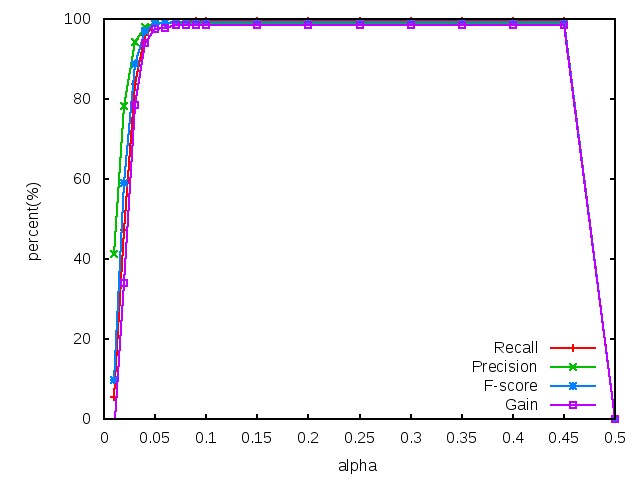
\includegraphics[width=0.5\textwidth]{alpha.jpg}
\caption{The effect of $\alpha$\label{fig:alpha}}
\end{center}
\end{figure}

If $\alpha$ is too small, too much solid kmers will be failed to get in table $A$ and too many positions will fail the hypothesis test. As a result, Lighter will try to correct those error-free region which also brings down the precision. And if $\alpha$ become even smaller, then there is no kmer in $B$, so Lighter will fail to correct all the reads because there is no candidate kmers. 

If $\alpha$ is larger, the hypothesis test is an adaptive threshold and handle this case nicely even if there are too many elements in $A$ and the false positive rate of $A$ is higher. However, when $\alpha$ is too large, the $k$-mer length $k$ will have a p-value larger than 0.005, and all the positions will be regarded as untrusted. We can observe this from the dramatic drop in Figure \ref{fig:alpha}.

This explanation can also be verified by looking at the occupancy rate of table A and B from the simulated data sets with 3 different coverage and $1\%$ error rate when changing $\alpha$ shown in Figure \ref{fig:bloom_occupancy_alpha_all}. Also, we can see the occupancy rate of table A is almost the same given the same $\alpha\times\mbox{coverage}$ across the 3 data sets. And the occupancy rate of table B is very steady because the solid kmers from the genome are the same for the 3 data sets. When $\alpha$ is way too large than the optimal value, like in the $140\times$ data set, too much weak kmers get sampled and more likely to pass the binomial test which cause the failure of filtering non-solid kmers.

\begin{figure}[h!]
\begin{center}
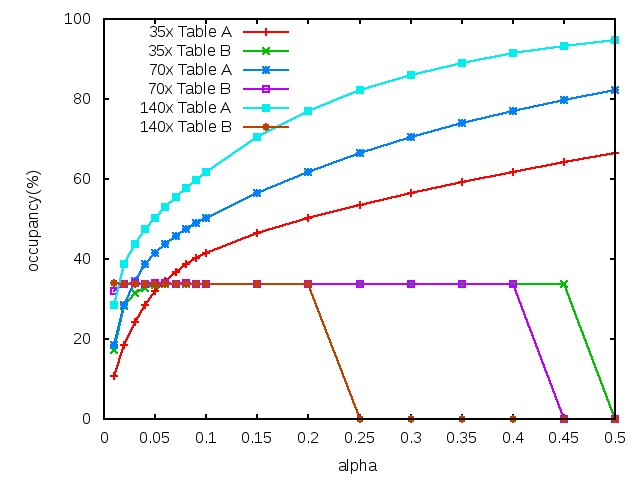
\includegraphics[width=0.5\textwidth]{bloom_occupancy_alpha_all.jpg}
\caption{The effect of $\alpha$ on occupancy rate\label{fig:bloom_occupancy_alpha_all}}
\end{center}
\end{figure}

One important parameters for $k$-mer based error correction methods is the value of $k$. When $k$ is too small, the $k$-mer containing sequencing error comes will likely be a $k$-mer from another location of the genome. When $k$ is too large, there may not be enough error-free $k$-mers for us to do error correction, especially when the coverage is not high. From the perspective of efficiency, when $k$ is large, we need more time to process a $k$-mer. And for the programs which requires storing the $k$-mer information, like using a hash table to store the counts, larger $k$ causes more memory consumption. Since Lighter does not store the $k$-mers' information explicitly, larger $k$ will only make Lighter slower but does not affect the memory usage.  In \cite{kelley2010quake}, the authors suggested that we can select $4^k$ around two hundred times the genome size. 

We measured the affect of $k$ using the simulated data set with $75\times$ coverage and $1\%$ error rate, the result is shown in Figure \ref{fig:kmerLength}. 

\begin{figure}[h!]
\begin{center}
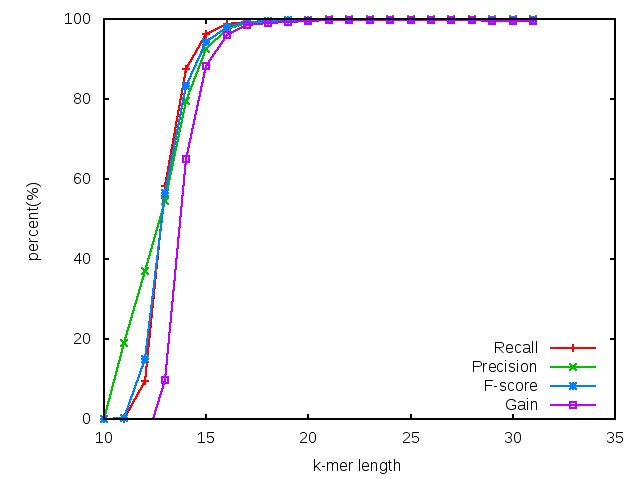
\includegraphics[width=0.5\textwidth]{kmerLength.jpg}
\caption{The effect of $\alpha$ on occupancy rate\label{fig:kmerLength}}
\end{center}
\end{figure}


\subsection*{Real data set}
\subsubsection*{E.Coli data set}
We use ERR022075 data set which is a very deep coverage sequencing data set of ecoli K-12 strain genome. We still used Quake, Musket, Bless and Lighter to run this data set. Since usually we do not need that much of coverage, we uniformly sampled some reads from this data set and got a data set with roughly 75x coverage. The reads in this data set is paired-end and the read length is 100 and 102. Because Bless can not handle paired-end reads with different length, we truncate the last 2 base to form a 100-length paired-end data set.

Since the genome of E.Coli K-12 strain is fully sequenced, we measured that 4,519,570 out of 4,553,699 kmers from the genome is stored in table $B$, which is more than $99\%$. This number can be slightly improved using larger $\alpha$. 
 
% Result of bowtie2
We can also measure the error corrections' effect on the alignment. We use Bowtie2[cite] to align the reads to the reference genome and count the total number of the matched position.

\begin{tabular}{|c|c|c|c||c|c|} \hline
	 & \multicolumn{3}{|c||}{Read Level} & \multicolumn{2}{|c|}{Base Level} \\ \hline
     & Total Reads 	& Mapped & Gain(\%) & Matched Pos & Gain(\%) \\ \hline
Original & 3,497,616 & 	99.04\%	 & - & 343,081,567	& - \\ \hline
Quake	& 3,369,584	& 99.98\%	& -2.75	& 327,813,255	& -4.45  \\ \hline
Musket	& 3,497,616	& 99.15\%	& 0.11	& 345,403,149	& 0.68  \\ \hline
Bless	& 3,497,616	& 99.30\%	& 0.26	& 345,947,230	& 0.84  \\ \hline
Lighter	 & 3,497,616	&  99.39\%	& 0.35	& 346,283,250	&  0.93  \\ \hline

\end{tabular}

For Quake, the number is very low mainly due to unreported reads and trimmed 3' end. It turns out Lighter gives the most improvement. We use samtools to do the SNP calling. 

For those reads not got trimmed and alinged to the genome without indels (cigar field like 100M in the SAM file), we measure the matched ratio for each position shown in Figure \ref{fig:ecoli_perbase}. Since many of the reads in this data set start with N, the first base's matching ratio of the original data set is very low.

\begin{figure}[h!]
\begin{center}
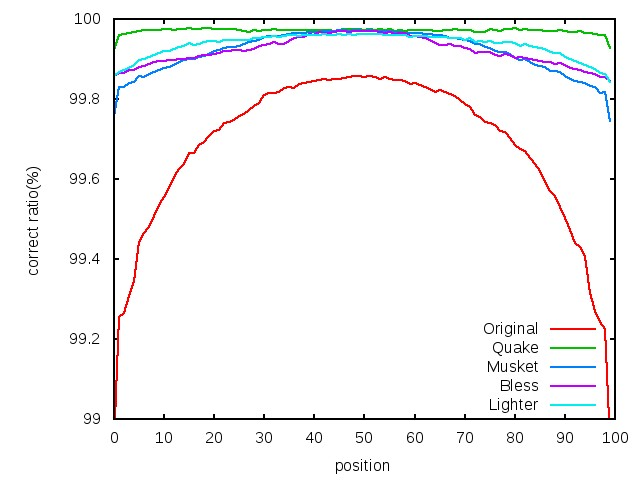
\includegraphics[width=0.5\textwidth]{per_base.jpg}
\caption{The matching ratio for each base in E.Coli data set\label{fig:ecoli_perbase}}
\end{center}
\end{figure}

% Result of SOAPDenovo2
Another common measurement for error correction is to run the de novo assembly and see the impact to the contigs. We use SOAPDenovo2[cite] to assemble the reads. SOAPDenovo2 is a de novo assembly software based on De Brujin graph. The parameter for SOAPDenovo2 especially the kmer size for the De Brujin graph is very important to the performance. We ran the SOAPdenovo2 on different parameters and choose the one with best N50 contig size for each program. Then for each chosen contig file, we evaluated the assembly quality using Quast[cite].

\begin{table}
\begin{tabular}{|c|c|c|c|c|c|} \hline
	 	& N50 &	L50	 & Mismatch / 100kbps&	Misassembly	& Coverage(\%) \\ \hline
Original	& 53584 & 28	& 0.31 &	0 &	98.289 \\ \hline 
Quake	& 54854	& 28	& 0.2	& 0	 & 98.248 \\ \hline
Musket	& 47826	& 31	& 3.53 &	0	& 98.244 \\ \hline
Bless	& 50573 & 	30	& 0.29	 & 0	& 98.276 \\ \hline
Lighter	&	47746	& 30	& 1.18 &0	& 98.261 \\ \hline
\end{tabular}
\caption{De novo assembly of E.Coli data set\label{table:ecoli_sd2}}
\end{table}

\subsubsection*{Human Chr14}
So far, we only tested the data on the genome of E.Coli, which is a pretty small. In this section, we use a data set from Gage[cite] on human chromosome 14. This data set is about 35x coverage and 101bp pair-end reads. And the $k$-mer size is 19 for all the programs in this data set.

Like for the E.Coli data set, we evaluate the result using both Bowtie2 and SOAPdenovo2.

The result of Bowtie2 is shown in Table \ref{table:chr14_bowtie2}.

\begin{table}
\begin{tabular}{|c|c|c|c||c|c|}\hline
  & \multicolumn{3}{|c||}{Read Level} & \multicolumn{2}{|c|}{Base Level} \\ \hline
  & Total Reads  & Mapped  &Gain(\%) &	Matched Pos	& Gain(\%) \\ \hline
Original &	36,504,800	& 98.60\%	&- &	3,581,034,345	& - \\ \hline
Quake &	32,560,518	& 99.96\%	& -9.57 &	3,040,192,216 &	-15.10 \\ \hline
Musket &	36,504,800 &	99.38\%	& 0.79	&3,631,477,901	& 1.41 \\ \hline
Bless &	36,504,800	&99.43\%	& 0.84	& 3,636,682,539 &	1.55 \\ \hline
Lighter	& 36,504,800	&99.37\% & 0.78	& 3,631,101,467	& 1.40 \\ \hline
\end{tabular}
\caption{Alignment of chr14 data set\label{table:chr14_bowtie2}}
\end{table}

% Result of SOAPDenovo2
We also tested the effect to de novo assembly using SOAPDeovo2 and Quast which is shown in Table \ref{table:chr14_sd2}. In this data set, the improvement due to error corrections is obviously. 

\begin{table}
\begin{tabular}{|c|c|c|c|c|c|} \hline
	   & N50 &	L50	& Mismatch / 100kbps &	Misassembly	& Coverage(\%) \\ \hline
Original &	3372 &	482	& 88.67	& 10 &	80.163 \\ \hline
Quake	& 3203	& 452 &	85.95 & 9 &	79.993 \\ \hline
Musket	& 3760	& 617 &	91.85 &	9 &	80.445 \\ \hline
Bless	& 3763	& 623 &	88.69 &	19 &	80.456 \\ \hline
Lighter	& 3766	& 618 &	90.22 &	12 &	80.498 \\ \hline
\end{tabular}
\caption{De novo assembly of chr14 data set\label{table:chr14_sd2}}
\end{table}

The results of the de novo assembly of the two real data set show that Lighter's result is comparable with other methods.

\subsection*{Running Time and Space Usage}
%describe the machine
The programs were run on a machine with 48 2.1GHz processors, 512G memory and 74T disk space. 

%The memory or disk usage from different programs 
Musket, Bless and Lighter are all aimming for low memory consumption. So we compared the peak memory usage as well as the peak disk consumption on the simulated data set with different coverage and with $1\%$ error rate and the chr14 real data from Gage.

\begin{tabular}{|c|c|c||c|c||c|c||c|c|} \hline
		& \multicolumn{2}{|c||}{$35\times$} & \multicolumn{2}{|c||}{$70\times$}  & \multicolumn{2}{|c||}{$140\times$} & \multicolumn{2}{|c|}{chr14}  \\ \hline
		& memory & disk & memory & disk & memory & disk & memory & disk \\ \hline
Quake   & 2.8G	& 3.3G & 7.1G & 6.0G & 14G & 12G & 48G & 57G \\ \hline		
Musket	& 139M	& 0 & 160M & 0 & 241M & 0 & 1.9G & 0 \\ \hline
Bless	& 10M	& 661M & 11M & 1.3G & 13M & 2.6G & 600M & 15G \\ \hline
Lighter	& 31M	& 0 & 31M & 0 & 31M & 0 & 510M & 0 \\ \hline
\end{tabular}

From the table, we can see that Bless and Lighter can achieve nearly constant memory consumption as claimed. Musket took much less memory comparing with Quake but is much worse than Bless and Lighter.

For Bless, we increase the number of temporary files along with the coverage of the data set to achieve the constant memory consumption. Bless uses secondary memory to save the memory consumption, and the overall space consumption is much larger than Musket and Lighter.  For the chr14 data set, The memory consumption of Bless can be decreased if we create more temporary files. 

%runtime on simulated_70_1
We compared the running time between Quake, Musket and Lighter using different number of threads on the simulated data set with $70\times$ coverage and $1\%$ error in Figure \ref{fig:runtime}. Musket requires at least 2 threads due to its master-slave style parallelism, so its figure start at when number of threads is 2. 

\begin{figure}[h!]
\begin{center}
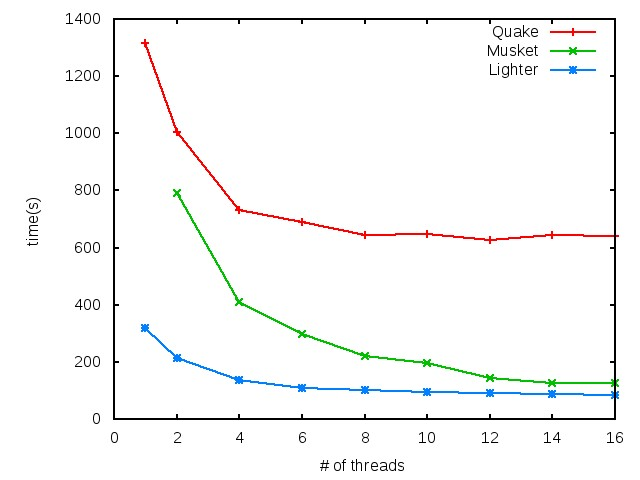
\includegraphics[width=0.5\textwidth]{runtime.jpg}
\end{center}
\caption{The running time on simulated data set with different number of threads\label{fig:runtime}}
\end{figure}

So far, Bless can only run in single-thread mode and it takes 1475s to finish which is much slower than Musket and Lighter.

The result shows that Lighter is very efficient and scalable. 

\section*{Discussion}
\emph{Lighter} is a software tool for correcting sequencing errors in sequencing datasets.
At \emph{Lighter}'s core is a method for obtaining a set of solid $k$-mers from a large collection of sequencing reads.
Unlike previous methods, \emph{Lighter} does this without counting $k$-mers in the reads.
By setting its parameters appropriately, its memory usage and accuracy can be held almost constant with respect to depth of coverage.
It is also quite fast and practical.

Though we demonstrate \emph{Lighter} in the context of sequencing error correction, \emph{Lighter}'s counting-free approach could be applied in other situation where a collection of solid $k$-mers is desired.
For example, one tool for scaling metagenome sequence assembly uses of a Bloom filter populated with solid $k$-mers as a memory-efficient, probabilistic representation of a De Bruijn graph \cite{pell2012scaling}.
Other tools use counting Bloom filters \cite{fan2000summary, bonomi2006improved} or the related CountMin sketch \cite{cormode2005improved} to represent De Bruijn graphs for compression \cite{jones2012compression} or digital normalization and related tasks \cite{zhang2013these}.
We expect Ideas from \emph{Lighter} could be useful in reducing the memory footprint of these and other tools. 

%We use this method to implement an error correction program Lighter for DNA-seq reads. As we expect, Light is space-efficient . Moreover, it is very fast and gives performance is comparable with other programs. This shows that our method of finding solid kmer is quite reliable. 

%Another immediate application of our method is getting solid kmers' count, which can be done by scanning the reads again to get the real count for the solid kmers stored in table $B$. 

%Since our method is probabilitic, we may miss few important information. Nevertheless, our method is extremely useful for programs like Quip[cite], where the accurate error correction is not critical. Even more, programs like Quip may directly use the solid kmers get by our method to do the assembly.

In this paper, we did not analyze the effect of $\alpha$ analytically and it is a difficult problem. So far, the size of table $A$ and $B$ are setting by considering unpractical pessimestic scenarios. If we know the effect in some compact form, we can optimize the performance of obtaining solid kmers by setting the best $\alpha$ and also use less space.

\emph{Lighter} is free open source software released under the XXX license.  The software and its source are available from \url{https://github.com/mourisl/Lighter/}.

%%%%%%%%%%%%%%%%%%%%%%%%%%%
\section*{Acknowledgements}
  Text for this section \ldots

\bibliographystyle{abbrv}
\bibliography{lighter_paper}

\end{document}







